\documentclass[12pt]{amsart}
\usepackage{amsmath, amssymb, amsthm, amscd, amsfonts}
\textwidth 6.5 in \oddsidemargin 0 in \evensidemargin 0 in
\textheight 8.5 in \topmargin 0in
\usepackage{pgfplots}
\pgfplotsset{width=10cm,compat=1.9}
\usepackage{url}
\usepackage{tikz}
\usepackage{graphicx}
\usepackage{wrapfig}
\usepackage{multicol}
\usepackage{oz}
\usepackage[
backend=biber,
style=science]{biblatex}
\usepackage{silence}
\usepackage{hyperref}
\usepackage{listings}
\usepackage{color}

\newcommand{\VV}{{\mathbb V}}
\newcommand{\RR}{{\mathbb R}}
\newcommand{\CC}{{\mathbb C}}
\newcommand{\ZZ}{{\mathbb Z}}
\newcommand{\QQ}{{\mathbb Q}}
\newcommand{\NN}{{\mathbb N}}
\newcommand{\EE}{{\mathbb E}}
\newcommand{\bfx}{{\bf x}}
\newcommand{\twodots}{\mathinner {\ldotp \ldotp}}

\newtheorem{question}{Question}
\newtheorem{axiom}{Axiom}
\newtheorem{theorem}{Theorem}[section]
\newtheorem{lemma}[theorem]{Lemma}
\newtheorem{corollary}[theorem]{Corollary}
\theoremstyle{definition}
\newtheorem{definition}[theorem]{Definition}
\newtheorem{notation}[theorem]{Notation}
\newtheorem{proposition}[theorem]{Proposition}
\newtheorem{problem}{Problem}
\newtheorem{objective}{Objective}
\newtheorem{example}[theorem]{Example}
\newtheorem{Algorithm}{Algorithm}
\theoremstyle{remark}
\newtheorem{remark}[theorem]{Remark}
\newtheorem{method}[theorem]{Method}
\newtheorem{exercise}{Exercise}

\definecolor{dkgreen}{rgb}{0,0.6,0}
\definecolor{gray}{rgb}{0.5,0.5,0.5}
\definecolor{mauve}{rgb}{0.58,0,0.82}

\lstset{frame=tb,
  language=Python,
  aboveskip=3mm,
  belowskip=3mm,
  showstringspaces=false,
  columns=flexible,
  basicstyle={\small\ttfamily},
  numbers=none,
  numberstyle=\tiny\color{gray},
  keywordstyle=\color{blue},
  commentstyle=\color{dkgreen},
  stringstyle=\color{mauve},
  breaklines=true,
  breakatwhitespace=true,
  tabsize=3
}

\bibliography{GANpaper}

\begin{document}

\title[Applications of Generative Adversarial Networks]{Applications of Generative Adversarial Networks to Natural Handwriting and Music Creation}

\thanks{
The authors, along with their advisor Dana Clahane, are partially supported by 
NSF-DMS-1541911: RE-C$^2$: Research Experiences in Community Colleges.
}

\author[K.Little]{Kyle Little}
\email{kylelittle2134@gmail.com}

\author[C.Stevens]{Christopher Stevens}
\email{cestevens@berkeley.edu}

\address{ Mathematics and Computer Science Division, \newline
        Fullerton College, 321 E. Chapman, Fullerton, CA 92832-2095
}

\begin{abstract}
We apply the recent concept of a generative adversarial network (GAN) to two tasks:
natural handwriting emulation and music creation. Because it is of great interest
to mathematically generalize neural networks (NNs), we will also present some 
abstract definitions that can serve as templates for NNs and GANs.
\end{abstract} 

\maketitle
\section{Introduction}

In this paper, we exhibit two applications of generative adversarial 
networks \cite{1406.2661}, and we attempt to generalize various aspects of them,
including the definition of a neural network. Before describing GANs, we will 
introduce some preliminary notation and definitions in the next sections. Later, 
we will proceed to applications of GANs in natural handwriting emulation and music 
creation. Because the generalization of neural networks is of great interest, 
along the way we will take the opportunity to propose general mathematical notions.
The reader will be provided with both code to the GANs and instructions for playing with our GANs.
We will also give some examples of outputs of our GANs in both applications.
For natural handwriting images are provided; for natural music creation
we provide links where MIDI files are stored so that the reader can perhaps be impressed.


\section{Definitions and Notation} 

Much of the mathematical probability and statistics preliminaries we include here
are borrowed from \citetitle{Clahaneprob}\cite{Clahaneprob}. We assume 
that the reader is familiar with the definition of a $\sigma$-field on a set $S$.
We also assume that the reader knows that a random variable is a function $X$ 
with domain in the sample space $S$ of a repeatable experiment and with co-domain
in a previously chosen set $T$. Suppose that ${\mathcal F}$ is a $\sigma$-field on a
set $S$. Let $P$ be a probability function on ${\mathcal F}$. Recall that $P$ 
and $X$ together induce a random variable $P_X$ on the collection of all inverse
images under $X$ of subsets of $T$ given by
\begin{equation*}
P_X(B):=P[X^{-1}(B)].
\end{equation*}
Note that this definition does not restrict us to the case when $X$ is a real 
variable. For example, $X$ could more generally, be vector-valued, matrix valued,
or operator valued.

Next, suppose that $X$ is a random variable that represents data that we have 
generated as a result of a collection and analysis algorithm. Then 
we may use $D$ in place of $X$ and denote $p_X$ instead by $p_{\text{data}}$.

If instead $X$ is a randomly generated noise variable $Z$, then we may use $Z$ 
as notation for $X$ and denote $p_Z$ instead by $p_z$ throughout the paper.


\begin{notation}[Prediction ($\sim$)]
        Let $m,n\in\NN$, and suppose that $\alpha\in[0,1]$. Let $S$ be a non-empty
        set for outcomes of some experiment or action. Suppose that ${\bf X}$ is 
        an $m\times n$-real matrix valued random variable on $S$; i.e., assume 
        that ${\bf X}:S\rightarrow M_{m\times n}$, where $M_{m\times n}$ denotes
        the collection of all real matrices of size $m\times n$. 
        Assume (for simplicity) that ${\bf X}$ is a continuous random variable. 
        Let $P$ be a probability function on a $\sigma$-field ${\mathcal F}$ on 
        $S$, and let $B\subset S$. Define the random variable $C_\alpha\circ{\bf X}$
        by $(C_\alpha\circ{\bf X})(s)=1$ if the probability that $s\in B$ is 
        $\geq \alpha$ and $(C_\alpha\circ{\bf X})(s)=0$ otherwise.
        
        Let $p_{\alpha,{\bf X}}$ more briefly denote the probability function induced 
        by $p$ and ${C_\alpha\circ \bf X}$. Let ${\bf X}_0\in {\bf X}(S)$.  Then the notation 
        ${\bf X}_0 \sim_\alpha p({\bf X}_0)$, or simply, ${\bf X}_0\sim p({\bf X}_0)$ 
        in the case that $\alpha=1/2$, denotes the phrase ``The value $p_{\alpha,X}({\bf X}_0)(s)$
        allows us to conclude that $s\in B$, with probability (i.e., the value of $p_{\alpha,{\bf X}}$) of truth of 
        this statement being $\geq \alpha$.''  Another way we may say this statement
        is, ``$p_{\alpha,{\bf X}}({\bf X}_0)(s)$ predicts $s$ is in $B$ with probability (i.e, value of $p_{\alpha,
        {\bf X}}[X_0(s)])$ being $\geq 1/2$."
\end{notation}

\begin{remark}
        Note, the entries of ${\bf X}(s)$ for some outcome $s\in S$ are called {\em predictors}.
\end{remark}

%\begin{example}  We consider a very simple application:  Suppose that ${\bf X}$ 
%is $Z$, the standard normally distributed real-valued random variable having mean
%$0$ and standard deviation $1$.  Suppose that $B$ here is $[0,\infty)$, and 
%suppose that our classification problem is that, once handed a datum value 
%$z\in\RR$, for example, $0.75$, we must predict if this number is in $B=[0,\infty)$
%using the standard normal cumulative distribution function.  
%Here, $P_Z:\RR\rightarrow[0,1]$ is given by
        %\begin{equation*}
        %P_Z(z)=\frac{1}{\sqrt{2\pi}}\integral_{-\infty}^z e^{-t^2}dt.
        %\end{equation*}
%In this case ${\mathcal F}$ is the Borel $\sigma$-field in $\RR$, which is the 
%intersection of all $\sigma$-fields that contain all of the open intervals in 
%$\RR$.  In particular, this $\sigma$-field contains any interval of the form 
%$(-\infty,z)$ where $z\in\RR$.  Then $0.75\sim_{1/2}P_Z(0.75)$ and 
%$0.75\sim P_Z(0.75)$ both denote the same statement, 
%``The value $P_Z(0.75)$ allows us to conclude that $0.75\in [0,\infty)$, 
%with probability of truth of this statement being $\geq 1/2$." In this 
%case $0.75$ is a predictor. The reader can verify,for example using a z-score 
%table, that $P_Z(0.75)$ is approximately $0.77337$. 
%
%Thus the statement that $0.75\sim P_Z(0.75)$ can be rewritten as $0.75\sim 0.77337$,
%which in turn means the same thing as the statement that the value $0.77337$ of 
%the cumulative distribution function here, the standard normal distribution 
%evaluated at $0.75$, indicates that $0.75\in[0,\infty)$, with probability $\geq 1/2$.
%\end{example}
%
To improve our predictions in the specific applications of GANs discussed in this
paper, we must first find how to quantify inaccuracy in our predictions. To do so,
we attempt to define an error function in the context of the above definition of
prediction. Later in this paper, we will specialize this idea to the more specific 
applications of Generative Adversarial Networks we are interested in, natural
handwriting and music creation.

\begin{definition}[Error Function] 
Let 
${\bf X}$ denote an $m\times n$-real matrix-valued (datum) variable that we would
like to use to classify whether or not a given outcome $s$ of an experiment is
or is not in a given set $B$ in the sample space $S$.  Let $P$ be a probability 
function on a $\sigma$-field ${\mathcal F}$ on $S$.  We say that a given function is an 
{\em error function induced by the variable ${\bf X}$ and $P$} and denote 
such  an error function by $\EE_{{\bf X}\sim{\bf P}({\bf X})}$if and only if the following
conditions are satisfied:
        \begin{enumerate}
                \item   
                    \begin{align*}
                        \EE_{{\bf X}\sim {\bf P}({\bf X})} : \RR \to \RR,
                    \end{align*}
                \item A given input $d\in\RR$ for this function is the output of
                    $f\circ P$, where $f$ is a one-to-one function on $[0,1]$,
                \item $\EE_{{\bf X}\sim{\bf P}({\bf X})}(d)=0$ when the input $d$
                    corresponds to the statement ${\bf X}\sim_1 P({\bf X})$;
                \item  A large value of $\EE_{{\bf X}\sim{\bf P}({\bf X})}(d)$ 
                    for some input $d$ corresponds to the statement that 
                    ${\bf X}\sim_\alpha P({\bf X})$ only for
                    small values of $\alpha\geq 0$.
        \end{enumerate}
\end{definition}



In order to make predictions, we must use some mathematical model. For the 
purpose of GANs, the model we will use is based on the human brain's layered 
neuron activity. We propose the following way of mathematically defining a 
neural network:

\begin{definition}[(Generalized) Neural Network]
    \leavevmode
    \begin{enumerate}
        \item We call $(V,E,W)$ a {\em neural network}, or more briefly an NN,
       if and only if the following statements hold:
        \begin{enumerate}
            \item $(V,E)$ is a digraph.
            \item $W$ is a function whose domain is $E$.
            \item $\forall (u,v)\in E$ such that $u$ is the terminal vertex 
            of an edge in $E$, we have that $u$ is a real number.
            \item $\forall (u,v)\in E$, $W(u,v):\ $Range$(u)\rightarrow$ Dom$(v)$.
        \end{enumerate}
        \item An NN $(V,E,W)$ is called {\em real-valued} if and only if $\forall (u,v)\in E$
        such that $v$ is the terminal vertex of an edge in $E$, we have that $v$ is a real number.
        \item Furthermore, the vertices of an NN that are both the terminal edge
        of a some vertex in $V$ and the initial edge of another vertex in $V$ are
        also called {\em neurons}.
    \end{enumerate}
\end{definition}

Recall that graphs can be connected or disconnected, or they can be simple or 
non-simple. Since an NN $(V,E,W)$ has an underlying graph $(V,E)$, then NNs can be
called connected, disconnected, simple, or non-simple, in exactly the same 
manner depending on the nature of the underlying graph.

However practically speaking, we note that in reasonable applications the 
underlying graph of an NN should be connected. Since an NN is a mathematical 
model inspired by how a brain works, a disconnected NN would be like two 
or more separate brains that don't interact with each other (not of interest in
this paper).  We remark that some neural networks, called recurrent ones, can 
have subgraphs of infinite length.  However, in the applications examined in this paper, 
recurrency is not a feature of our GAN's.

For the applications that we are interested in, the vertices of a given 
neural network that are functions will have domains and ranges in Euclidean space.

\begin{definition}[Euclidean NN and notation within it]
    \leavevmode
    \begin{enumerate}
        \item We call an NN $(V,E,W)$ {\em Euclidean} if and only if each $v\in V$ is either
        a real constant or $v:\RR^m\rightarrow\RR^n$ for some positive integers 
        $m,n$ and, $\forall (u,v)\in E$, we have that $W(u,v)$ is either a real 
        number or a column vector of real numbers whose number of components is 
        the same as the dimension of the domain of $v$. 
        
        \item Let $(V,E,W)$ be an Euclidean NN, and let $v\in\mathbb{N}$ be the 
        cardinality of $V$. Denote the vertices by $v_1,v_2,\ldots, v_k$. 
        \begin{enumerate}
                \item We denote by $I:=\{0\twodots k\}$, the set of all integers
                    between and including $0$ and $k$. 
                \item With respect to $m_0,m_1, m_2, \dots, m_k, n_0, n_1, n_2, 
                    \dots, n_k \in \mathbb{W}$, the set of all positive integers, we impose that 
                    $m_i$ $\forall i$ is the dimension of the domain of $v_i$ vertex 
                    and also impose that $n_i$ is the dimension of the range of $v_i$.
                \item That is, we suppose that each vertex $v_i$ of $V$ here satisfies
                    \begin{align*}
                        v_i:\mathbb{R}^{m_i} \to \mathbb{R}^{n_i} 
                    \end{align*}
                \item If $i,j\in \{1..k\}$ and $(v_i,v_j)\in E$, then we denote 
                    $W(v_i,v_j)$ more briefly by $w_{i,j}$.
        \end{enumerate}
    \end{enumerate}
\end{definition}

The weights we assign each neuron change the network's influence on these neurons.
Sometimes, we do not want a neuron to be included in the calculation for training
so the network does not gain dependency on one neuron. Analogously to the human 
brain we have certain neurons removed from the graph.

\begin{remark}[Drop-out]
        A weight of zero represents a vertex or neuron has {\em dropped-out} for
        some training cycle. Since the weight is a scalar multiplied by the input
        vector, when that weight is zero, that input will be ignored.
\end{remark}

\begin{definition}[Perceptron]
        A {\em perceptron} is a neural network consisting of a single layer of 
        weights and with identity functions as the vertex set.
\end{definition}

\begin{remark}
        As an effect of this definition, perceptrons may be modeled as linear 
        predictors, or as functions ${\bf q}(\bfx)\sim {\bf p}(\bfx)$. Later in 
        the paper we will use this notation to refer to perceptrons.
\end{remark}

We define neural networks as above to create a general mathematical structure for
the theory of a largely implementation-based algorithm. Allowing each neuron to 
be any function and generalizing weights allows for a general theoretical neural
network definition. A GAN uses two neural networks which are consequently trained
in tandem. We will define the two separate neural networks before we define the 
full GAN.

\begin{definition}[Discriminator]
        A {\em discriminator} is a type of neural network that determines 
        authenticity of input data. It can be modeled by a function 
        $$ D:\RR^n \to \RR, $$ together with the other properties of a more 
        general NN.
\end{definition}

The discriminator is a neural network that takes a vector to check if 
it is part of the same set as the data it was trained on. 
It outputs a probability that the vector is a part of its training set.

\begin{definition}[Generator]
        A {\em generator} is a type of neural network that produces
        new data based on training, and can be described as a function
        $$ G:{\bf z} \to \RR^n $$
        where ${\bf z}$ is a noise vector.
\end{definition}

The generator is some neural network that takes in some kind
of random noise and outputs things that look like the training
data. Thus, when we train our generator in tandem with our
discriminator we can evoke the idea of counterfeiting, in the
sense that the outputs of the generator try to fool
the input to the discriminator.

\section{Definition of a Generative Adversarial Network}

\begin{definition}[Generative Adversarial Network]
        We define a {\em generative adversarial network} (GAN) in terms of a
        two player min-max game between a discriminator $D$ and a
        generator $G$ with value function
        \begin{align*}
                \min\limits_{G}\max\limits_{D}V(D,G) = \mathbb{E}_{{\bf x} \sim p_{data}({\bf x})}[\log D({\bf x})] + 
                \mathbb{E}_{{\bf z} \sim p_{{\bf z}}({\bf z}) } \left[ \log(1-D(G({\bf z}))) \right]\text{  \cite{1406.2661}}
        \end{align*}
        where we train $D$ to maximize the probability of correctly assigning
        labels to both training data and data that comes from $G$. In turn we train $G$
        to minimize $\log(1-D(G({\bf z})))$.
\end{definition}

\section{Results}
\subsection{Natural Handwriting}

In the first application of GANs we attempted to produce handwritten letters and
numbers in a manner that looks human written. We achieved partial results,
based upon and modified from open source work by Diego Gomez\footnote{https://github.com/diegoalejogm/gans}.
Many changes were made in order to preserve outputs long term, as well
as laying foundations for cohesive data inputs. For example, work was first
done using MNIST as the input data, which produced very legible numbers. \\
\begin{center}
    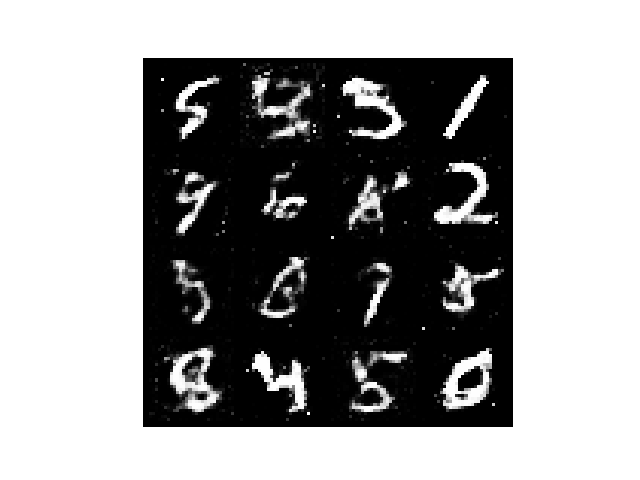
\includegraphics[scale=0.5]{output1.png} \\
\end{center}
The code for the handwriting portion and instructions on how to run it can be found at
\href{https://github.com/Onionchi/GANdwriting}{https://github.com/Onionchi/GANdwriting}

Listed here is an example in Python of how to train an actual neural network.

\small{
\begin{lstlisting}
for epoch in range(num_epochs):
  for n_batch, (real_batch,_) in enumerate(data_loader):

    # 1. Train Discriminator
    real_data = Variable(images_to_vectors(real_batch))
    if torch.cuda.is_available(): real_data = real_data.cuda()
    # Generate fake data
    fake_data = generator(noise(real_data.size(0))).detach()
    # Train D
    d_error, d_pred_real, d_pred_fake = 
            train_discriminator(d_optimizer, real_data, fake_data)

    # 2. Train Generator
    # Generate fake data
    fake_data = generator(noise(real_batch.size(0)))
    # Train G
    g_error = train_generator(g_optimizer, fake_data)
    # Log error
    logger.log(d_error, g_error, epoch, n_batch, num_batches)

    # Display Progress
    if (n_batch) % 100 == 0:
      display.clear_output(True)
      # Display Images
      test_images = vectors_to_images(generator(test_noise)).data.cpu()
      logger.log_images(test_images, num_test_samples,
                        epoch, n_batch, num_batches);
      # Display status Logs
      logger.display_status(
        epoch, num_epochs, n_batch, num_batches,
        d_error, g_error, d_pred_real, d_pred_fake
      )
    # Model Checkpoints
    logger.save_models(generator, discriminator, epoch)
\end{lstlisting}
}

\subsection{Music Creation}
With the second application of GANs we attempted to produce new music based upon 
MIDI files from various classical composers. This involved two neural network models
over the course of our research. Both of these models were useful in finding out more about GANs.
Outputs to both models were generally not similar to music that would be considered "normal,"
but there was significant improvement between the two models. The model is based off starting code, 
which was originally an MNIST GAN that we heavily modified.
\footnote{https://skymind.ai/wiki/generative-adversarial-network-gan}

The first model was a naive implementation of a GAN. This model simply took the
input MIDI files and tried to produce new MIDI files that were similar. This led to results that generally fit in one
of two categories.
\begin{enumerate}
    \item The MIDI file output would be a jumble of notes equivalent to someone randomly pushing 
        keys on a keyboard.
    \item The MIDI file output would degrade into two notes one very high pitched and the other very low
        pitched. These notes would repeat at seemingly random intervals throughout.
\end{enumerate}

We think that these two outcomes are due to a phenomenon known as modal collapse. More specifically over the process
of training GANs, they will sometimes learn only one way of making output as indicated above.

The second model has many improvements over the first. The parameter that used to be a raw note value
was changed to be a difference between notes over time. This way the neural network could try to learn
some form of structure over time in music. This change was very successful and brought about new MIDI
output that had segments resembling musical scales and arpeggios that might be features of human composed music.
The following code includes the pre--processing performed on the data to add a note difference algorithm.
\small{
\begin{lstlisting}
#Input: MidiFile Object, Output: Ordered Matrix with each part representing a note
def make_midi_matrix(mid_in, data_out):
    global min_time, max_time, min_channel, max_channel, min_note, max_note, min_attack, max_attack
    first_loop = True #If we are in the first loop we will say the note is zero and store the note to get the difference 
    for track in mid_in.tracks:
        for msg in track:
            if not first_loop:
                if not msg.is_meta and msg.type == "note_on":
                    command = (msg.channel, msg.note-prev_note, msg.velocity, msg.time) #Get the note difference
                    min_time = min_time if min_time <= msg.time else msg.time
                    max_time = max_time if max_time >= msg.time else msg.time
                    min_channel = min_channel if min_channel <= msg.channel else msg.channel
                    max_channel = max_channel if max_channel >= msg.channel else msg.channel
                    data_out.append(command)
                    prev_note = msg.note
            else:
                if not msg.is_meta and msg.type == "note_on":
                    command = (msg.channel, 0, msg.velocity, msg.time) #Init line one with a note base of 0
                    first_loop = False
                    min_time = min_time if min_time <= msg.time else msg.time
                    max_time = max_time if max_time >= msg.time else msg.time
                    min_channel = min_channel if min_channel <= msg.channel else msg.channel
                    max_channel = max_channel if max_channel >= msg.channel else msg.channel
                    prev_note = msg.note #Save the current cycles note for differences
    return data_out
\end{lstlisting}
}

The above code and more is available at
\href{https://github.com/Aniranth/GAN_Project}{https://github.com/Aniranth/GAN\_Project}.
Simply get Python 3 on your system and follow the instructions in 
the README file of the GitHub. You can also find sample MIDI files 
generated by several epochs of testing of the GAN at this link. The data used 
was acquired courtesy of \href{http://www.jsbach.net/midi/}{http://www.jsbach.net/midi/}
and \href{http://www.shiningsilence.com/hpr/misc/}{http://www.shiningsilence.com/hpr/misc/}


\section{Further Research}
There are many different directions that can be taken for further research.
Currently for the application of handwriting we are trying to emulate the handwriting
of Thomas Jefferson, as he has a large volume of annotated written work, available at
the Library of Congress.

We would like to look further into the modal collapse that was experienced in the
Music application. The authors would specifically like to consider a paper found
late in the research as this paper developed.\cite{1809.09087}

Another project the authors have significant personal interest in will be to
implement the more generalized neural network that outputs functions rather than
real numbers.

\section{Acknowledgements}
Kyle Little would like to thank Ryan Wilcox for his suggestion to use a change 
in notes for the note predictor in the second version of the Music application for GANs.

Christopher Stevens would like to thank David Nuon for his helpful conversations
about different types of neural networks. These conversations helped inspire thought about 
neural networks in the non-traditional view expressed in this paper.

As well, we would like to thank Kevin Scully for several wonderful talks about 
neural networks at the Fullerton College Mathematics Colloquium, which inspired 
our selection of this data science topic for the current project, and for
reading over a draft of this paper and giving some useful advice. 

The authors would like to thank Professors Helena Noronha, Bruce Shapiro, and 
Adriano Zambom of California State University Northridge for their work organizing
this research project and their
lectures on data science. The authors would also like to thank the Department 
of Mathematics at California State University Northridge  for providing 
hospitality and for hosting the Math Research Experiences in Community 
Colleges Conference  for the past three years.

Both authors would also like to give special thanks to their research advisor Dr. Dana Clahane
for both his help throughout this project and for the inspiration to pursue research while
still in community college.

This project was completed as part of Research Experiences in Community Colleges (REC$^2$), 
which has been funded by the National Science Foundation, 
under Division of Mathematical Sciences Grant Number 1541911.

\newpage

\printbibliography

\end{document}
